\chapter{Teoretické východiská}
\label{kap:teoria}

V tejto kapitole sa venujeme základným pojmom a kľúčovým konceptom potrebným pre vývoj autonómnych agentov v hernom prostredí Trackmania. Zameriame sa na umelú inteligenciu a strojové učenie, vrátane rôznych typov učenia, ako sú učenie pod dohľadom, učenie bez dohľadu a učenie posilňovaním. Vysvetlíme aj dôležité koncepty, ako sú neurónové siete a ich štruktúra, ktoré sú základom moderných systémov umelej inteligencie. Ďalej sa budeme venovať počítačovej grafike, ktorá pomôže modelovať virtuálne prostredie pre agentov a simulovať senzory. Na záver sa zameriame na autonómne riadenie vozidiel a na samotnú hru Trackmania.

\section{Umelá inteligencia}
\label{sec:umela_inteligencia}

Zakladateľ informatiky, Alan Turing, sa v jednej z jeho prác zamýšľal nad otázkou, či dokážu stroje rozmýšľať \cite{turing_machinery_and_inteligence}. V tejto práci tvrdil, že počítače majú potenciál simulovať ľudské zmýšľanie, ako napríklad hrať šach. Pár rokov na to, v roku 1956, John McCarthy tento okruh informatiky pomenoval ako umelá inteligencia \cite{history_of_AI}. Jedná sa o jednu z najviac skúmaných oblastí informatiky, hlavne kvôli rozsiahlosti riešených problémov. Tieto problémy sa pohybujú od exaktných, ako je prehľadávanie grafov, cez robotiku, napodobňovanie ľudského zmýšľania a správania, autonómne riadenie vozidiel až po filozofické otázky, či sa stroje iba tvária ako inteligentné, alebo naozaj rozmýšľajú \cite{artificial_intelligence_modern_aproach}.

Ak si však položíme otázku, čo to vôbec umelá inteligencia je, odpovede sa môžu líšiť podľa literatúry \cite{history_of_AI, artificial_intelligence_modern_aproach, ai_in_games_brief_review}. Vo všeobecnosti chápeme pojem umelá inteligencia ako systém, ktorý sa snaží napodobňovať charakteristiky ľudského zmýšľania a následne vyvodzovať vlastné rozhodnutia, učiť sa alebo premýšľať bez ľudského zásahu \cite{artificial_intelligence_modern_aproach}. Aj napriek tomu, že si ľudia často predstavujú umelú inteligenciu ako robota z budúcnosti, podľa definície môže byť umelá inteligencia aj jednoduchý program, ktorý pomocou pravidiel charakterizuje určité správanie \cite{ai_in_games_brief_review}.

\subsection{Agent}

V oblasti umelej inteligencie pojmom agent označujeme čokoľvek, čo dokáže vnímať svoje okolie pomocou senzorov a interagovať s prostredím pomocou efektorov \cite{artificial_intelligence_modern_aproach}. Tak, ako človek má oči, uši a ďalšie orgány na sledovanie svojho okolia, taktiež má aj časti tela ako ruky, nohy a hlas na interagovanie s prostredím. Podobne robot môže mať kameru, hĺbkové senzory, mikrofón na sledovanie svojho okolia a rôzne motory, reproduktory či časti robota môžu slúžiť ako efektory. V tomto prípade môžeme takéhoto robota považovať za agenta. Stav agentových senzorov v hociakom momente nazývame vnem; história všetkého, čo agent kedy vnímal, je postupnosť vnemov \cite{artificial_intelligence_modern_aproach}.

Matematicky môžeme agenta a jeho rozhodovanie popísať ako funkciu $\pi$, ktorá mapuje postupnosť vnemov (historické údaje) na akciu:
\[
\pi: (s_1, s_2, \ldots, s_t) \rightarrow a_t
\]
kde $s_t$ je stav prostredia v čase $t$ a $a_t$ je akcia zvolená agentom \cite{artificial_intelligence_modern_aproach}.

\subsection{Racionálne správanie}

Agenta môžeme považovať za inteligentného, keď na ľubovoľný stav prostredia reaguje správne. Toto je síce jednoduchý koncept, ktorý my ľudia chápeme prirodzene, správna reakcia je určite lepšia ako nesprávna, avšak čo to vlastne znamená reagovať správne? Aby sme zistili, či si agent v prostredí počína dobre, musíme si definovať kritérium hodnotenia, podľa úlohy, ktorú agent vykonáva. Úlohou agenta je následne získať čo najlepšie hodnotenie. Ak sa agentovi podarí splniť naše kritériá, potom tohto agenta môžeme považovať za racionálneho.\cite{artificial_intelligence_modern_aproach}.

Formálne môžeme kritérium hodnotenia popísať ako funkciu odmeny $R$, ktorá závisí od stavu prostredia $s_t$ a akcie $a_t$:
\[
R(s_t, a_t)
\]
Úlohou agenta je maximalizovať kumulatívnu odmenu:
\[
\sum_{t=0}^{T} R(s_t, a_t)
\]

\subsection{Špecifikácia úlohy pre agenta}

Už sme si vysvetlili pojmy pre agenta ako prostredie, senzory, efektory a kritérium hodnotenia. Pri navrhovaní agenta musíme jasne popísať problematiku, teda jednoznačne pomenovať každý vymenovaný aspekt a popísať, kedy budeme považovať agenta za racionálneho \cite{artificial_intelligence_modern_aproach}.

Ako príklad môžeme použiť problematiku pretekárskeho auta a pokúsime sa popísať agenta:

\begin{itemize}
\item  typ agenta – šofér pretekárskeho auta,
\item  prostredie – pretekárska dráha,
\item  senzory – kamera, LiDAR senzor,
\item  efektory – zatáčanie, plyn, brzda,
\item  kritérium hodnotenia – prejsť trať v čo najkratšom čase, nebúrať.
\end{itemize}


%% =============================================================================
\section{Strojové učenie}
\label{sec:strojove_ucenie}

Strojové učenie je vetva umelej inteligencie, ktorá sa zaoberá vývojom algoritmov, ktoré umožňujú počítačom učiť sa zo získaných dát bez explicitného programovania \cite{artificial_intelligence_modern_aproach}. Tradičný program zahŕňa pravidlá a inštrukcie pre počítač, pričom algoritmus je popísaný exaktne. Naopak, strojové učenie dokáže identifikovať vzorce správania zo získaných dát. Tento prístup používame pre riešenie problémov, ktoré sú príliš komplexné na to, aby sme ich dokázali popísať tradičnými algoritmami. Klasický príklad pre túto problematiku je rozpoznávanie obrazu. Ak by sme chceli rozpoznávať na obrázku objekt ako automobil, veľmi ťažko by sme dokázali spraviť tradičný program, ktorý by vedel rozpoznávať automobil na obrázku. Tento zložitý problém preto najčastejšie riešime pomocou strojového učenia, kde z veľkého množstva dát rozpoznáme spoločné črty pre automobil.

\subsection{Typy strojového učenia}

Strojové učenie možno rozdeliť do troch hlavných kategórií, podľa toho, ako učenie prebieha a podľa typu dát, ktoré máme k dispozícii \cite{artificial_intelligence_modern_aproach} TODO vymenovať aj.

\begin{enumerate}
\item \textbf{Učenie pod dohľadom (Supervised learning)}

Tento typ učenia využíva označené dáta, kde ku každému vstupu máme priradený požadovaný výstup. Cieľom tohto učenia je naučiť model rozpoznávať vzorce z trénovacej množiny dát a následne pre neoznačené dáta predpovedať správny výstup. V praxi si tento typ učenia môžeme predstaviť tak, že modelu dáme obrázky, na ktorých sa auto nachádza alebo nenachádza, pričom ku každému obrázku bude priradené správne označenie, či sa na ňom auto nachádza alebo nie. Následne, ak by sme tomuto modelu dali nový obrázok, ktorý ešte nevidel, mal by nám správne povedať, či sa jedná o obrázok auta alebo nie. Tento prístup sa však nemusí obmedzovať iba na jednoduché rozhodovacie problémy ako je prítomnosť auta, ale môže byť použitý aj na zložitejšie úlohy, napríklad identifikáciu typu auta na obrázku (klasifikácia) \cite{artificial_intelligence_modern_aproach}.

Matematicky, učenie pod dohľadom hľadá funkciu $f$, ktorá mapuje vstupy $X$ na výstupy $Y$, kde $\epsilon$ je šum v dátach:
\[
Y = f(X) + \epsilon
\]

\item \textbf{Učenie bez dohľadu (Unsupervised learning)}

Pri učení bez dohľadu sú dáta neoznačené a cieľom je nájsť skryté štruktúry alebo vzorce v dátach \cite{artificial_intelligence_modern_aproach}. Tento typ učenia je užitočný pre rozdelenie množiny do skupín. Príkladom môže byť klasifikácia zákazníkov na základe ich nákupného správania. Predstavme si, že máme databázu obsahujúcu históriu nákupov od tisícok zákazníkov, pričom nevieme, aké typy zákazníkov v tejto databáze existujú. Pomocou učenia bez dohľadu, konkrétne použitím metódy zhlukovania (clustering), môžeme analyzovať tieto dáta a identifikovať rôzne skupiny zákazníkov s podobným nákupným správaním. Napríklad môžeme zistiť, že existujú skupiny zákazníkov, ktorí pravidelne nakupujú elektroniku, iní zas preferujú módu a ďalší často nakupujú potraviny. Takéto rozdelenie nám umožňuje lepšie pochopiť rôzne typy zákazníkov a prispôsobiť marketingové stratégie pre jednotlivé skupiny.

\item \textbf{Učenie posilňovaním (Reinforcement learning)}

Ide o špecifický typ učenia, kde agent interaguje s dynamickým prostredím, v ktorom sa snaží maximalizovať dlhodobý zisk \cite{reinforcment_learning_intro}. Učenie posilňovaním z veľkej časti odráža našu definíciu agenta, kde agent vníma prostredie pomocou senzorov, interaguje s prostredím pomocou efektorov a snaží sa maximalizovať výsledky podľa kritéria hodnotenia \cite{artificial_intelligence_modern_aproach}. 
Tento typ učenia môžeme prirovnať k Pavlovovým psom. V experimente, ktorý vykonal Ivan Pavlov, pss reagovali na zvonenie zvončeka slinením, pretože si zvuk spojili s príchodom potravy. Podobne, v učení posilňovaním sa agent učí vykonávať akcie na základe odmien alebo trestov, ktoré dostáva po vykonaní žiaducej alebo nežiaducej akcie. Tento typ učenia sa využíva v oblastiach ako hranie videohier, navigácia robotov po priestore alebo v oblasti autonómnych vozidiel, kde agent musí spraviť sériu rozhodnutí, ktoré vedú k úspechu alebo zlyhaniu \cite{reinforcment_learning_intro}.

\end{enumerate}

\subsection{Evolučné algoritmy a neuroevolúcia}

Evolučné algoritmy sú inšpirované biologickými evolučnými procesmi a používajú sa na optimalizáciu a hľadanie riešení v komplexných problémoch \cite{artificial_intelligence_modern_aproach}. Neuroevolúcia, konkrétne NEAT (NeuroEvolution of Augmenting Topologies), je metóda, ktorá využíva evolučné algoritmy na trénovanie neurónových sietí. NEAT je schopný nielen optimalizovať váhy v neurónovej sieti, ale aj dynamicky meniť topológiu siete, čo znamená pridávanie nových neurónov a spojení počas evolúcie \cite{neat_article}.

Matematicky môžeme neuroevolúciu popísať ako optimalizačný problém, kde cieľom je nájsť optimálnu štruktúru a váhy neurónovej siete $N$ pre danú úlohu:
\[
\text{argmax}_{N} \sum_{t=0}^{T} R(s_t, a_t)
\]
kde $R(s_t, a_t)$ je odmeňovacia funkcia závislá na stave prostredia $s_t$ a akcii $a_t$.

NEAT začína s jednoduchými sieťami a postupne evolvuje ich štruktúru pomocou genetických operácií ako kríženie a mutácia. Tento prístup umožňuje zachovať výhody jednoduchej siete v počiatočných fázach učenia a zároveň umožňuje postupné zložitejšie prispôsobenie sa komplexným úlohám \cite{neat_article}.


\section{Odmeňovacia funkcia (Reward function)}

Pri učení posilňovaním musíme mať jasne stanovený cieľ, ktorý agent musí dosiahnuť \cite{reinforcment_in_real_time}. Podľa stanoveného cieľa dokážeme rozhodnúť, či si agent v prostredí počína správne alebo nesprávne. Napríklad ak agent nikdy nedosiahne cieľ, nemali by sme ho odmeňovať, a naopak, ak agent cieľ dosiahne, mal by získať veľkú odmenu. Agentovým cieľom v učení posilňovaním je maximalizovať súčet hodnôt tejto odmeňovacej funkcie \cite{reinforcment_in_real_time}. Odmeňovacia funkcia môže byť dvoch základných typov:

\textbf{Finálna odmena}

Agent nedostane počas celého pokusu žiadnu spätnú väzbu, či si počína dobre alebo nie, až v momente keď dosiahne cieľ, prípadne spraví rapídnu chybu, dostane pozitívnu alebo negatívnu odmenu. Tento prístup má výhody v jasnom stanovení cieľa a jednoznačnosti rozhodnutia, či si agent počínal dobre alebo nie. Avšak podľa zložitosti úlohy môže byť dosiahnutie cieľa pre agenta takmer nemožné, čím nikdy nezíska žiadnu spätnú väzbu k jeho správaniu. Je možné, že agent nikdy nenájde globálne maximum pre funkciu rozhodovania, keďže nikdy nedosiahne cieľ \cite{reinforcment_learning_intro}.

\textbf{Čiastková odmena}

Agent dostáva odmenu počas celého pokusu, čím ihneď získava spätnú väzbu, či si počína dobre. Táto odmena je väčšinou aproximácia toho, či sa agent priblížuje k cieľu. Tento prístup má aj negatívny dopad a to ten, že agent ľahko napreduje k maximalizovaniu odmeny, avšak ľahko môže uviaznuť do lokálneho maxima, kde sa naučil dobre maximalizovať čiastkovú odmenu, ale cieľ nedosiahne, alebo ho dosiahne iba s horšími okolnosťami \cite{reinforcment_learning_intro}.


\textbf{Hybridný prístup}

Oba prístupy majú svoje výhody a nevýhody. Ak je to možné, vždy je lepšie použiť prístup s finálnou odmenou, aby sme sa vyhli neoptimálnemu riešeniu. Ak sa však agent nedokáže v rozumnom čase naučiť dosiahnuť cieľ, je možné mu pomôcť čiastkovou odmenou a správne ho nasmerovať. Počas tréningu je možné odmeňovaciu funkciu zmeniť. Preto je niekedy potrebné začať s čiastkovou odmenou, ktorú v neskorších fázach tréningu zameníme za finálnu odmenu \cite{reinforcment_learning_intro}.



%% ================================================================================================
\section{Neurónové siete}
\label{sec:neuronove_siete}

Neurónové siete sú jedným z kľúčových nástrojov v oblasti strojového učenia, inšpirované biologickými procesmi v ľudskom mozgu. Sú zložené z vrstiev neurónov, kde každý neurón je jednoduchá spracovateľská jednotka pracujúca s dátami vstupujúcimi do siete. Tieto siete sa učia transformovať vstupné dáta na požadované výstupy prostredníctvom procesu, ktorý zahŕňa prispôsobovanie váh spojení medzi neurónmi. Tréning neurónovej siete zvyčajne prebieha pomocou metódy nazývanej spätné šírenie (backpropagation), kde chyby vo výstupoch sú použité na upravenie váh tak, aby siete mohli presnejšie predpovedať výsledky. Tieto siete sa osvedčili pri riešení rôznych úloh, ako je rozpoznávanie obrazu, spracovanie prirodzeného jazyka a predikcia sekvenčných dát, vďaka ich schopnosti zachytávať komplexné vzťahy a vzorce v dátach. Na základe svojej všestrannosti a efektivity sú neurónové siete dnes dominantnou technológiou v mnohých pokročilých aplikáciách umelej inteligencie \cite{artificial_intelligence_modern_aproach, end_to_end_self_driving}.

\subsection{Matematika neurónových sietí}

Jednou z najdôležitejších vlastností neurónových sietí je fakt, že dokážu aproximovať ľubovoľnú funkciu \cite{artificial_intelligence_modern_aproach}. Neurónovú sieť môžeme matematicky popísať ako zloženie funkcií:
\[
y = f(x) = f^{(n)}(f^{(n-1)}(\cdots f^{(1)}(x)\cdots))
\]
kde $f^{(i)}$ je funkcia aplikovaná v $i$-tej vrstve siete. Každá vrstva transformuje vstup pomocou váh a aktivačnej funkcie:
\[
z^{(i)} = W^{(i)} a^{(i-1)} + b^{(i)}
\]
\[
a^{(i)} = \sigma(z^{(i)})
\]
kde $W^{(i)}$ sú váhy, $b^{(i)}$ sú prahové hodnoty (bias), $z^{(i)}$ je lineárna transformácia a $\sigma$ je nelineárna aktivačná funkcia, napríklad logistická sigmoida $\sigma(z) = \frac{1}{1 + e^{-z}}$ \cite{artificial_intelligence_modern_aproach}.

\subsection{Konvolučné neurónové siete}

Konvolučné neurónové siete (CNNs) sú špecifickým typom neurónových sietí, ktoré sú obzvlášť účinné pri spracovaní obrazových dát \cite{artificial_intelligence_modern_aproach}. Základným stavebným prvkom CNN je konvolučná vrstva, ktorá aplikuje konvolučnú operáciu na vstupný obraz. Matematicky je konvolúcia definovaná ako:
\[
S(i,j) = (I * K)(i,j) = \sum_m \sum_n I(m,n) K(i-m, j-n)
\]
kde $I$ je vstupný obraz, $K$ je konvolučný filter a $S$ je výstupný obraz. Konvolúcia umožňuje extrakciu lokálnych vzorov v obraze, ako sú hrany, rohy alebo textúry \cite{krizhevsky2012imagenet}.

\subsection{Hlboké neurónové siete}

Hlboké neurónové siete (DNNs) sú neurónové siete s mnohými skrytými vrstvami. Tieto siete dokážu zachytávať veľmi komplexné vzťahy v dátach, čo im umožňuje riešiť zložité úlohy \cite{goodfellow2016deep}. Tréning DNNs často prebieha pomocou gradientného zostupu, kde cieľom je minimalizovať funkciu chyby (napríklad Mean Squared Error):
\[
E = \frac{1}{2N} \sum_{i=1}^N (y_i - \hat{y}_i)^2
\]
kde $y_i$ je skutočný výstup a $\hat{y}_i$ je predikovaný výstup siete. Aktualizácia váh prebieha podľa pravidla:
\[
W \leftarrow W - \eta \frac{\partial E}{\partial W}
\]
kde $\eta$ je učebný krok a $\frac{\partial E}{\partial W}$ je gradient chyby vzhľadom na váhy \cite{goodfellow2016deep}.


%% ================================================================================================
\section{Autonómne riadenie vozidiel}
\label{sec:autonomne_auta}

Čoraz častejšie môžeme na ulici vidieť vozidlo, ktoré sa po cestách pohybuje bez ľudského zásahu. Takéto vozidlá nazývame autonómne. Ide o vozidlá, ktoré sú schopné vykonávať všetky riadiace funkcie bez potreby ľudskej interakcie. Kľúčovými cieľmi vývoja autonómnych vozidiel sú zvýšenie bezpečnosti na cestách, pohodlie ľudí, ale aj menej viditeľné dopady ako zníženie emisií \cite{autonomous_vehicle_goals}. Jedná sa však o veľmi zložitú problematiku, keďže nedokážeme pomocou jednoduchých pravidiel definovať správanie sa vozidla na cestách. Aj napriek tomu, že máme zákony o cestnej premávke, tieto pravidlá stačia pre ľudí, ktorí chápu abstrakciu a popísanie problémov na vysokej úrovni. Avšak popísať počítaču, čo má robiť v ľubovoľnom okamihu jazdy, je takmer nemožné. Preto sa na riešenie tohto problému často používajú neurónové siete. Tak, ako sme vyššie spomenuli, namiesto toho aby sme popísali správanie exaktne, pokúsime sa funkciu čo najlepšie aproximovať. Autonómne vozidlo môžeme považovať za agenta, ktorý vníma svoje okolie pomocou senzorov, podľa ktorých robí rozhodnutia a interaguje so svetom pomocou efektorov. Vďaka neurónovým sieťam dokážu autonómne vozidlá plynule reagovať na dynamické prostredie cestnej premávky, čo je zásadné pre ich bezpečné a efektívne fungovanie. Bez týchto pokročilých algoritmických riešení by integrácia autonómnych vozidiel do každodennej dopravy nebola možná \cite{autonomous_vehicle_goals}.

\subsection{Senzory}

Ľudia sú vizuálne tvory, ktoré viac ako 90\% informácií vnímajú pomocou zraku \cite{gregory1979eye}. Samozrejme, nemôžeme zabúdať na sluch, hmat, čuch, ktoré nám pri šoférovaní môžu pomôcť. Pomocou sluchu môžeme vnímať výstrahy ako klaksón alebo sirény. Pomocou čuchu môžeme detekovať poruchu na aute alebo v okolí a pomocou hmatu môžeme cítiť hrboly na ceste alebo nárazy. Je nám však jasné, že bez zraku by sme v žiadnom prípade nedokázali plnohodnotne riadiť vozidlo. Ľudský pár očí okrem samotného obrazu dokáže vnímať aj hĺbku a určiť, ako ďaleko od očí sa objekty nachádzajú. Analogicky, aby sa autonómne vozidlo dokázalo správne rozhodovať, potrebuje byť vybavené rôznymi senzormi, ktoré umožňujú dostatočne vnímať okolie \cite{end_to_end_self_driving}. Najčastejšie sa stretávame s týmito senzormi:

\textbf{Kamery:} Zaznamenávajú vizuálne informácie, podobne ako ľudské oko. Sú kľúčové pre detekciu cestných značiek, semaforov a iných vozidiel na ceste \cite{end_to_end_self_driving}.

\textbf{Hĺbkové senzory:} Aj napriek tomu, že pomocou viacerých kamier by sme dokázali získať informácie o vzdialenosti objektov, tento proces by bol veľmi zložitý a výpočtovo náročný. Preto sa na získanie vzdialeností okolitých objektov používajú hĺbkové senzory, ktoré fungujú na princípe vysielania vĺn a počítania odrazu lúča. Tento spôsob je rýchlejší a presnejší ako počítanie vzdialeností z viacerých kamier \cite{end_to_end_self_driving}.

\textbf{GPS:} Ľudia sa dokážu orientovať po cestách podľa pamäti. Pre automobil by však bolo nemožné pamätať si každý stav, v ktorom sa kedy nachádzal. Autonómne vozidlo by sa tak mohlo dostať do situácie, na ktorú by nevedelo správne reagovať. Z tohto dôvodu je veľkou časťou vnímania okolitého prostredia, okrem lokálnych informácií z kamier a hĺbkových senzorov, aj globálna informácia z GPS. Spolu s použitím máp dokáže autonómne vozidlo naplánovať trasu do cieľovej destinácie \cite{end_to_end_self_driving}.

%% ============================================================================================
\section{Počítačová grafika}
\label{sec:grafika}

Počítačová grafika je oblasť informatiky, ktorá sa zaoberá zobrazovaním trojrozmerných geometrických objektov a scén na dvojrozmernú obrazovku. Za týmto zdanlivo jednoduchým procesom sa skrýva veľa technických výziev. Počítačová grafika sa využíva hlavne v oblastiach videohier, virtuálnej a rozšírenej reality či vo filmovom priemysle alebo simuláciách \cite{computer_graphics}. 

\subsection{Zobrazovanie objektov a koncept scény}

V počítačovej grafike sú objekty často reprezentované ako súbor dátových bodov v 3D priestore, ktoré definujú ich geometriu. Scéna v počítačovej grafike sa odvoláva na kompletné digitálne prostredie, ktoré obsahuje všetky objekty, svetelné zdroje, kamery a ďalšie grafické prvky potrebné pre finálne zobrazenie. Scéna je v podstate „svet“, v ktorom sa všetky tieto prvky nachádzajú a interagujú. Vykreslovanie (rendering), ktorý transformuje 3D modely do 2D obrazov, simuluje, ako svetlo interaguje s objektmi v scéne, vrátane vytvárania tieňov, odrazov a iných vizuálnych efektov, ktoré prispievajú k realistickému vzhľadu \cite{computer_graphics}.

\subsection{Dátová reprezentácia objektu}

V počítačovej grafike poznáme viac reprezentácií objektu. Jedna z najpoužívanejších je však reprezentácia pomocou trojuholníkovej mriežky (3D mesh). Jedná sa o dátovú štruktúru, ktorá obsahuje vrcholy v trojrozmernom priestore a hrany medzi vrcholmi, ktoré vytvárajú trojuholníky. Pomocou týchto trojuholníkov dokážeme do určitej presnosti napodobniť zložité objekty \cite{computer_graphics}.

Matematicky môžeme objekt reprezentovať ako množinu trojuholníkov $\{T_i\}$, kde každý trojuholník $T_i$ je definovaný svojimi vrcholmi $\{v_1, v_2, v_3\}$.

\subsection{Raycasting}

Pojem raycasting v počítačovej grafike opisuje proces vysielania lúčov z bodu do scény na určenie viditeľnosti alebo vzdialenosti objektu z daného bodu. Jedná sa o podobný mechanizmus ako ten, ktorým LiDAR senzory detekujú objekty v reálnom svete prostredníctvom emitovania laserových lúčov a merania ich odrazov. Raycasting si teda môžeme v jednoduchosti predstaviť ako vystrelenie laserového lúču z ľubovoľného bodu v scéne. Tento mechanizmus má veľkú výhodu v efektívnosti, keďže počítame prienik roviny trojúholníka a priamky, čo je pre počítač iba riešenie rovnice v asymptotickej zložitosti \(O(1)\). Musíme však myslieť na to, že týchto trojúholníkov sa v scéne nachádza \(N\), teda výpočet prieniku lúča so scénou dokážeme robiť v zložitosti \(O(N)\) \cite{computer_graphics}.

Matematicky je raycasting definovaný ako riešenie rovnice:
\[
\mathbf{r}(t) = \mathbf{o} + t\mathbf{d}
\]
kde \(\mathbf{r}(t)\) je lúč v čase \(t\), \(\mathbf{o}\) je počiatočný bod lúča a \(\mathbf{d}\) je smerový vektor lúča. Úloha raycastingu je nájsť prienik tohto lúča s objektmi v scéne.


%% ==============================================================================================
\section{Virtuálne prostredie}
\label{sec:virtualne_prostredie}

Virtuálne prostredie predstavuje svet mimo našej reality, kde môžeme trénovať autonómne vozidlo. Tieto prostredia ponúkajú simulované podmienky, ktoré umožňujú vývojárom bezpečne experimentovať, meniť systémy či algoritmy bez rizík, ktoré môžu vzniknúť v reálnom svete. Medzi hlavné výhody virtuálneho prostredia patria \cite{ai_in_games_brief_review}:

\begin{itemize}
\item  Bezpečnosť: Virtuálne prostredie eliminuje riziko nehôd, umožňujúc bezpečné testovanie vozidiel v extrémnych alebo nebezpečných situáciách. Tento aspekt má veľkú úlohu pri učení posilňovaním, keďže tento prístup je svojím spôsobom “pokus-omyl”. Je takmer nemožné trénovať autonómne vozidlo posilňovaním v reálnom svete. 
\item  Modifikovateľnosť: Pri trénovaní autonómneho vozidla potrebujeme agenta vystaviť čo najrozmanitejším scenárom, aby bol agent schopný vykonať adekvátne rozhodnutie počas krízových situácií. Ak nám prostredie umožňuje veľkú mieru modifikovateľnosti, dokážeme generovať veľké množstvo trénovacích dát, ktoré by v reálnom svete neboli možné.
\item  Opakovateľnosť: Experimenty vo virtuálnom prostredí sú ľahko reprodukovateľné, čo umožňuje lepšie vyladenie chýb alebo porovnávanie rôznych prístupov či algoritmov.
\item  Efektívnosť: Simulácie umožňujú rýchle iterovanie medzi experimentami. 
\item  Úspornosť: Ak by sme sa aj pokúsili trénovať autonómne vozidlo v reálnom svete, dochádzalo by k opotrebovaniu súčiastok a možno aj k poškodeniam vozidla. Preto je nákladovo efektívnejšie autonómne vozidlo trénovať najskôr vo virtuálnom prostredí.
\end{itemize}

Hlavne kvôli týmto výhodám sa častokrát stretávame s postupom, kedy autonómne vozidlo trénujeme najskôr vo virtuálnom prostredí a až keď je auto úspešne natrénované, systém implementujeme do fyzického vozidla, kde tréning pokračuje \cite{ai_in_games_brief_review}.

\subsection{Výber virtuálneho prostredia}

Pri výbere vhodného prostredia na trénovanie autonómnych vozidiel je nevyhnutné zohľadniť niekoľko faktorov. Prvým z nich je realistické a presné modelovanie fyzikálnych vlastností vozidla a okolia. Dôležité je, aby virtuálne prostredie dokázalo poskytnúť dostatočný počet rôznorodých a významných situácií, s ktorými sa autonómne vozidlo môže stretnúť. Okrem toho by malo mať aj flexibilné možnosti modifikácie a prispôsobenia, čo umožní rozširovanie a úpravu trénovacích scenárov podľa konkrétnych potrieb. \cite{ai_in_games_brief_review}

%% =================================================================================================
\section{Trackmania}
\label{sec:trackmania}



Trackmania je pretekársky simulátor, ktorý kladie veľký dôraz na precízne ovládanie vozidla pri vysokých rýchlostiach s cieľom dosiahnuť najlepší čas prejdenia trate. Pre dokončenie trate musí hráč najskôr prejsť cez všetky kontrolné brány, pričom ich môže prejsť v akomkoľvek poradí a následne dosiahnuť cieľovú bránu \cite{trackmania_is_np}. Tento príncíp môžme lepšie pochopiť z obrázka \ref{obr:track}.

Trackmania má viacero verzií ako Trackmania: Nations Forever, Trackmania: United, alebo najnovšia verzia Trackmania 2020. Princíp hry je vo všetkých verziách rovnaký a fyzika vozidla takmer totožná, preto sa zameriame na najnovšiu verziu Trackmania 2020 \cite{trackmania_is_np}.


\begin{figure}
%vlozenie samotneho obrazku vycentrovaneho a vhodnej velkosti
%obrazok je v subore images/cervik.png
\centerline{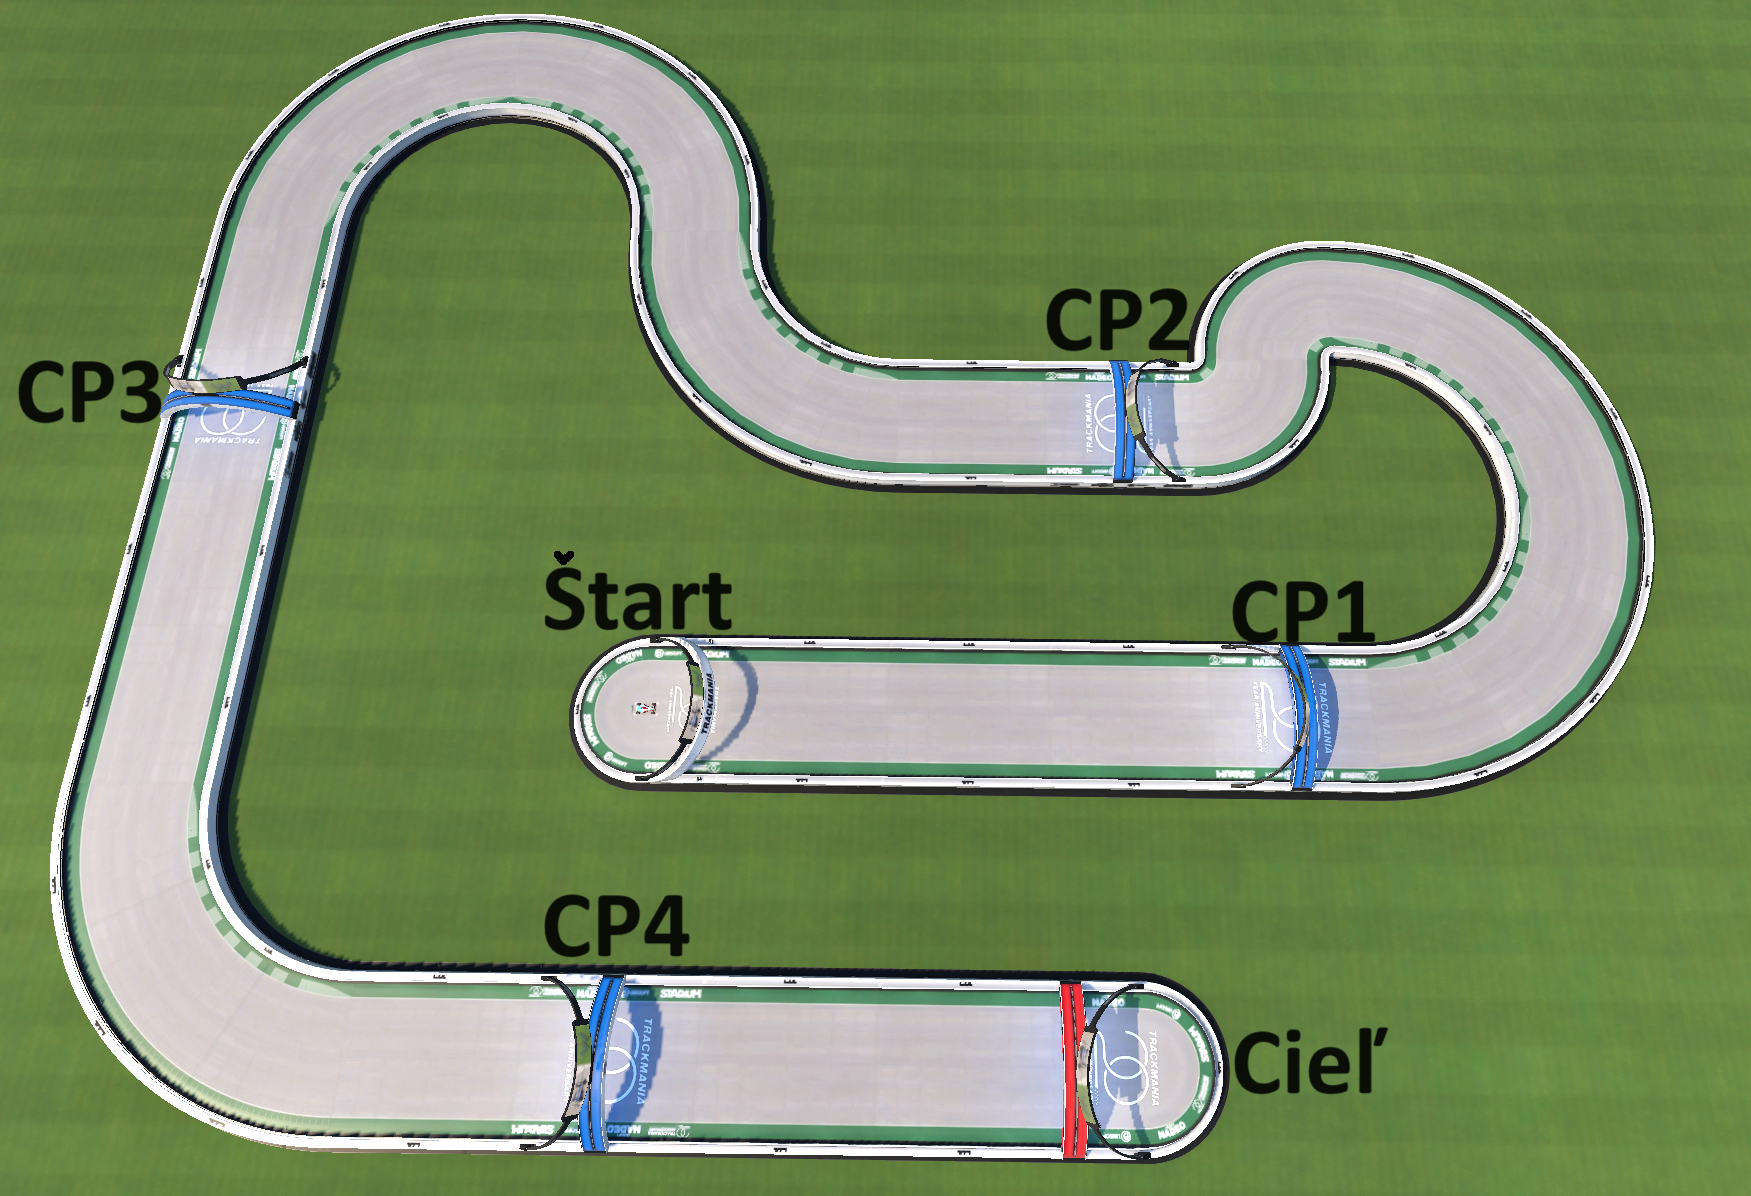
\includegraphics[width=0.5\textwidth]{images/track.png}}
%popis obrazku
\caption[Ukážka trate]{Na obrázku môžme vidieť pôdorys jednoduchej trate v hre Trackmania. Môžme si všimnúť, že mapa okrem štartu a cieľa obsahuje niekoľko kontrolných brán.}
%id obrazku, pomocou ktoreho sa budeme na obrazok odvolavat
\label{obr:track}
\end{figure}

Jedným z významných aspektov Trackmanie je jej deterministický charakter. To znamená, že rovnaký vstup od hráča vždy vedie k rovnakému výsledku. Tento fakt robí Trackmaniu ideálnym prostredím pre trénovanie hlbokých neurónových sietí. Umožňuje opakovateľné experimenty a presné vyhodnocovanie výkonu a zlepšenia algoritmov riadenia vozidiel \cite{trackmania_is_np}.

Ďalšou významnou charakteristikou Trackmanie je jej vysoká kompetitívnosť. Hráči sú motivovaní súperiť o každú stotinu sekundy a dosiahnuť čo najlepší výsledok. Vďaka tejto konkurencii je hra dynamická a náročná na zručnosť a rýchle rozhodovanie. Pre trénovanie umelej inteligencie je táto vysoká úroveň súťaže výzvou, ktorú je potrebné zohľadniť pri vytváraní riadiacich algoritmov.

Trackmania nám ponúka výhodu v tvorbe vlastných tratí, čo predstavuje významný aspekt hry. Hráči majú slobodný prístup k vytváraniu rôznorodých tratí s rôznymi konfiguráciami a stupňami obtiažnosti. Trate sú zostavené z viacerých blokov, ktoré disponujú rôznymi povrchmi, ako sú asfalt, hlina, ľad, tráva a mnoho ďalších. Každý povrch ovplyvňuje jazdné vlastnosti vozidla. Tieto bloky môžu mať rôzne veľkosti, tvary a pozície na mape, čo môžme vidieť na obrázku \ref{obr:editor_options}. Vďaka veľkému množstvu kombinácií týchto blokov je k dispozícii mnoho tisícok trás, ktoré boli vytvorené rôznymi hráčmi. Každá trať je sprevádzaná záznamami najlepších časov, čo poskytuje bohatý a rozmanitý dataset, ideálny pre trénovanie a testovanie umelej inteligencie.

\begin{figure}
%vlozenie samotneho obrazku vycentrovaneho a vhodnej velkosti
%obrazok je v subore images/cervik.png
\centerline{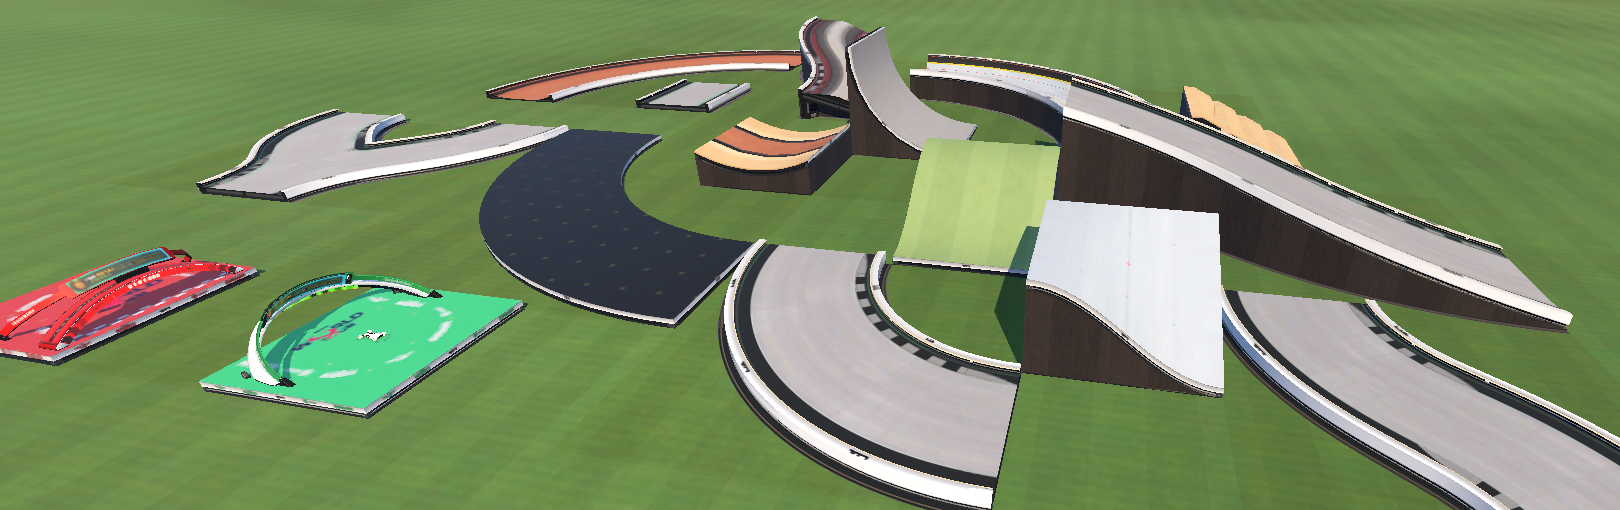
\includegraphics[width=1\textwidth]{images/editor.png}}
%popis obrazku
\caption[Paleta blokov]{Obrázok ilustruje rozmanitosť povrchov a tvarov blokov, pričom hra Trackmania ponúka stovky rôznych blokov na tvorbu herných máp.}
%id obrazku, pomocou ktoreho sa budeme na obrazok odvolavat
\label{obr:editor_options}
\end{figure}

\subsection{Openplanet}

Openplanet je open-source platforma, ktorá rozširuje funkcionalitu samotnej hry Trackmania. Je to voľne dostupný softvér, ktorý umožňuje hráčom interagovať s hrou a vytvárať vlastné skripty pomocou jazyka AngelScript, ktorý je podobný programovaciemu jazyku C. Openplanet umožňuje komunikáciu s herným enginom Trackmanie a poskytuje programátorské rozhranie (API), ktoré využijeme na extrahovanie dát v reálnom čase. Pomocou API je možné získať dáta ako pozícia automobilu na mape alebo rýchlosť a smer pohybu. Na komunikáciu so samotnou platformou Openplanet môžeme použiť ľubovoľný programovací jazyk, ktorý umožňuje komunikáciu pomocou TCP/IP protokolu \cite{tmrl_github}. 


